\subsection{Phân hệ quản lý công tác}
\label{subsec:business_trip}

\subsubsection{Mục tiêu}
Công tác là một trong những nghiệp vụ quan trọng hỗ trợ người lao động toàn trường tối
ưu quá trình quản lý thông tin quy trình các chuyến đi công tác. Quy trình quản lý thông tin công tác bắt đầu từ việc
đăng ký công tác của cán bộ. Đơn đăng ký công tác sẽ được gửi đến các bên liên quan để thẩm định và phê duyệt, người dùng cũng nắm bắt được thông tin về tiến độ các bước phê duyệt.
Sau khi được phê duyệt, cán bộ sẽ thực hiện chuyến công tác và báo cáo kết quả (nếu có).


\subsubsection{Yêu cầu chức năng}

\begin{table}[H]
\centering
\small
\caption{Yêu cầu chức năng nhóm quản lý công tác}
\label{tab:fr_business_trip}
\begin{tabularx}{\textwidth}{|L{1.8cm}|L{3.5cm}|L{2.5cm}|Y|}
\hline
\textbf{Mã FR} & \textbf{Chức năng} & \textbf{Tác nhân} & \textbf{Mô tả và ràng buộc nghiệp vụ} \\
\hline
FR-BTR-01 & Tra cứu đơn & Cán bộ, Giảng viên & Xem danh sách đơn công tác cá nhân, lọc theo trạng thái và xem chi tiết tiến trình duyệt. \\
\hline
FR-BTR-02 & Tạo và gửi đơn & Cán bộ, Giảng viên & Tạo phiếu đăng ký công tác, điền thông tin và gửi cho các bên liên quan phê duyệt. \\
\hline
FR-BTR-03 & Quản lý nháp và điều chỉnh & Cán bộ, Giảng viên & Chỉnh sửa hoặc xóa phiếu Nháp; chỉnh sửa và gửi lại phiếu Bị trả lại. Người lập không tự thu hồi phiếu đã gửi. \\
\hline
FR-BTR-04 & Xử lý đơn & Các bên liên quan & Xem xét thông tin đơn đăng ký, minh chứng và thực hiện các thao tác như: phê duyệt, từ chối hoặc trả lại đơn theo thẩm quyền. \\
\hline
FR-BTR-05 & Thu hồi đơn & Chuyên viên P.TCNS/BGH & Thu hồi đơn đăng ký công tác ở bất kỳ bước nào trong quy trình. \\
\hline
\end{tabularx}
\end{table}

\subsubsection{Đặc tả Use Case}
\begin{figure}[H]
    \centering
    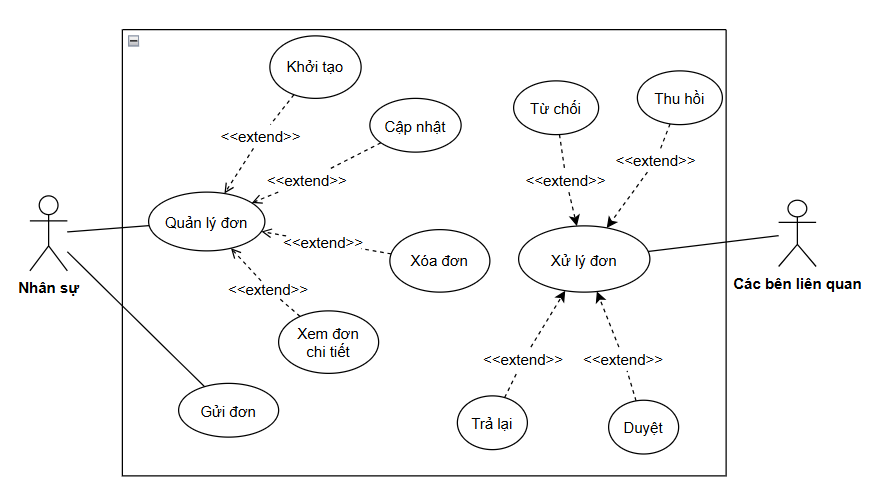
\includegraphics[width=\linewidth]{image/usecase/UC_BT.png}
    \caption{\textit{Sơ đồ use-case quản lý công tác}}
    \label{fig:BT_UC}
\end{figure}

\usecasespec{
    id={UC-BT-01},
    name={Soạn thảo đơn đăng ký công tác},
    actor={Cán bộ / Giảng viên},
    pre={Đã đăng nhập vào ứng dụng và tài khoản có quyền tạo đơn đăng ký công tác.},
    trigger={Người dùng chọn biểu tượng tạo mới đơn đăng ký công tác trên ứng dụng.},
    mainflow={
            1. Hệ thống khởi tạo đơn ở trạng thái nháp (\texttt{DRAFT}). \newline
            2. Người dùng nhập thông tin qua biểu mẫu từng bước: chọn khoảng thời gian, hình thức (trong nước, nước ngoài), phân loại (cá nhân, đoàn), địa điểm, kinh phí, đính kèm minh chứng (nếu cần), .... \newline
            3. Người dùng nhấn nút "Lưu" đơn đăng ký công tác. \newline
            4. Hệ thống lưu lại thông tin đã nhập và đơn có trạng thái là "Nháp". \newline
        },
    altflow={
            1.1. Chọn đơn đăng ký công tác từ danh sách các đơn đã tạo có trạng thái là "Nháp" hoặc "Trả lại", hệ thống hiển thị thông tin chi tiết của đơn. Thực hiện tiếp bước 2. \newline
        },
    post={Đơn ở trạng thái nháp (\texttt{DRAFT}) hoặc trả lại (\texttt{RETURNED}).},
    label={tab:uc_bt_01}
}


\usecasespec{
    id={UC-BT-02},
    name={Gửi đơn đăng ký công tác},
    actor={Cán bộ / Giảng viên},
    pre={Đã đăng nhập vào ứng dụng và tài khoản có quyền tạo đơn đăng ký công tác.},
    trigger={Người dùng chọn đơn đăng ký công tác có trạng thái là "Nháp" hoặc "Trả lại"},
    mainflow={
            1. Người dùng nhấn nút gửi đơn đăng ký công tác. \newline
            2. Hệ thống kiểm tra tính hợp lệ của thông tin nhập vào. \newline
            3. Hệ thống kiểm tra lịch trình cá nhân để rà soát xem có trùng lịch với các hoạt động khác không. \newline
            4. Hệ thống tạo quy trình phê duyệt tương ứng với thông tin của đơn đăng ký công tác và thêm vào lịch cá nhân của các thành viên tham gia. \newline
            5. Hệ thống gửi đơn đăng ký công tác đến các bên liên quan để thẩm định và phê duyệt. \newline
            6. Hệ thống khóa lịch trình cá nhân và thông báo cho các bên liên quan. \newline
            7. Người dùng truy cập đơn đăng ký công tác để xem thông tin chi tiết, trạng thái phê duyệt, lịch sử thao tác.
        },
    exflow={
            2.1. Tại bước 2, nếu thông tin nhập vào không hợp lệ, hệ thống thông báo lỗi và yêu cầu người dùng chỉnh sửa. \newline
            3.1. Tại bước 3, nếu có trùng lịch trình cá nhân, hệ thống thông báo lỗi và yêu cầu người dùng chỉnh sửa lại thời gian công tác. \newline
        },
    post={Đơn đăng ký công tác được gửi đến các bên liên quan để thẩm định và phê duyệt.},
    label={tab:uc_bt_02}
}

\usecasespec{
    id={UC-BT-03},
    name={Xóa đơn đăng ký công tác},
    actor={Cán bộ / Giảng viên},
    pre={Đã đăng nhập vào ứng dụng, là người lập đơn và đơn đang ở trạng thái Nháp.},
    trigger={Người dùng truy cập vào danh sách đơn đăng ký công tác.},
    mainflow={
            1. Người dùng chọn đơn đăng ký công tác có trạng thái là "Nháp" để xóa. \newline
            2. Người dùng nhấn nút "Xóa" để xóa đơn đăng ký công tác. \newline
            3. Hệ thống hiển thị hộp thoại xác nhận xóa đơn đăng ký công tác. \newline
            4. Người dùng xác nhận xóa đơn đăng ký công tác. \newline
            5. Hệ thống kiểm tra đơn vẫn ở trạng thái Nháp, sau đó xóa đơn đăng ký công tác.
        },
    exflow={
            5.1. Nếu đơn đã được gửi hoặc thay đổi trạng thái, hệ thống từ chối xóa và giữ nguyên dữ liệu.
        },
    post={Chỉ đơn Nháp hợp lệ được xóa khỏi hệ thống.},
    label={tab:uc_bt_03}
}

\usecasespec{
    id={UC-BT-04},
    name={Phê duyệt đơn đăng ký công tác},
    goal={Cho phép cán bộ có thẩm quyền tại từng cột mốc xem xét và đưa ra quyết định (Duyệt / Trả lại / Từ chối) đối với phiếu công tác đã được gửi, đưa phiếu đi qua chuỗi các cấp thẩm định phù hợp với loại công tác cho đến khi được Ban Giám hiệu phê duyệt chính thức hoặc bị chấm dứt.},
    actor={Lãnh đạo đơn vị, Lãnh đạo Phòng KH\&CN, Chuyên viên/ Lãnh đạo TC-NS, Văn phòng Ban Giám hiệu, Ban Giám hiệu},
    pre={
            - Đơn đã được gửi và đang ở một trong các bước duyệt: \texttt{TRUONG\_DV}, \texttt{KHCN}, \texttt{CV\_TCNS}, \texttt{TP\_TCNS}, \texttt{CV\_BGH}, \texttt{BGH}. \newline
            - Người thực hiện có thẩm quyền duyệt tại đúng bước hiện tại của phiếu
        },
    trigger={Người duyệt mở phiếu đang chờ tại bước của mình và chọn một trong ba hành động: Duyệt, Trả lại, Từ chối.},
    mainflow={
            1. Lãnh đạo đơn vị mở phiếu đang chờ duyệt tại bước \texttt{TRUONG\_DV}. \newline
            2. Người duyệt xem xét thông tin chuyến đi, thời gian vắng mặt, phương án phân công thay thế. \newline
            3. Người duyệt chọn "Duyệt". \newline
            4. Hệ thống chuyển phiếu sang bước tiếp theo và ghi nhật ký quy trình (người duyệt, thời gian duyệt). \newline
            5. Hệ thống gửi thông báo đến cán bộ có thẩm quyền duyệt ở bước kế tiếp. \newline
        },
    altflow={
            5.1. Tại bước 5, nếu phiếu đang ở bước duyệt cuối cùng (\texttt{BGH}), hệ thống chuyển phiếu sang trạng thái \texttt{KET\_THUC}. \newline
            A2 — Trả lại phiếu: \newline
            3.2. Người duyệt chọn "Trả lại" và nhập ghi chú yêu cầu chỉnh sửa. \newline
            4.2. Hệ thống sẽ trả lại phiếu cho người nộp và mở lại quyền chỉnh sửa cho người nộp. \newline
            5.2. Hệ thống gửi thông báo kèm ghi chú cho người nộp. \newline
            A3 — Từ chối phiếu: \newline
            3.3. Người duyệt chọn "Từ chối" và nhập ghi chú lý do từ chối. \newline
            4.3. Hệ thống cập nhật trạng thái phiếu thành \texttt{TU\_CHOI}. \newline
            5.3. Hệ thống giải phóng toàn bộ lịch cá nhân đã khóa của các thành viên tham gia. \newline
            6.3. Hệ thống thông báo cho người nộp và mọi thành viên liên quan. \newline
        },
    post={Đơn chuyển sang trạng thái mới thành công.},
    label={tab:uc_bt_04}
}

\usecasespec{
    id={UC-BT-05},
    name={Thu hồi đơn đăng ký công tác},
    actor={Chuyên viên/Lãnh đạo Phòng TCNS, Văn phòng BGH},
    pre={Đã đăng nhập vào ứng dụng và tài khoản có quyền thu hồi đơn đăng ký công tác.},
    trigger={Người dùng truy cập vào danh sách đơn đăng ký công tác.},
    mainflow={
            1. Người dùng chọn đơn đăng ký ở bất kỳ trạng thái nào. \newline
            2. Người dùng nhấn nút "Thu hồi" để thu hồi đơn đăng ký công tác. \newline
            3. Hệ thống hiển thị hộp thoại xác nhận thu hồi đơn đăng ký công tác. \newline
            4. Người dùng xác nhận thu hồi đơn đăng ký công tác. \newline
            5. Hệ thống cập nhật trạng thái phiếu thành "Đã thu hồi" (\texttt{REVOKED}) và giải phóng lịch trình cá nhân đã khóa của các thành viên tham gia. \newline
            6. Hệ thống thông báo cho người nộp và mọi thành viên liên quan về việc thu hồi phiếu.
        },
    post={Đơn chuyển sang trạng thái "Đã thu hồi" (\texttt{REVOKED}).},
    label={tab:uc_bt_05}
}

\subsubsection{Quy tắc nghiệp vụ}
\begin{itemize}
    \item \textbf{BR-BT-01:} Quy trình phê duyệt công tác mặc định là: Duyệt cấp đơn vị → Chuyên viên TC-NS → Lãnh đạo TC-NS → Văn phòng BGH → Ban Giám hiệu.
    \item \textbf{BR-BT-02:} Nếu thông tin phiếu có kinh phí là "Kinh phí KHCN", hệ thống sẽ thêm bước thẩm định của Phòng KHCN trước khi chuyển sang Phòng TC-NS.
    \item \textbf{BR-BT-03:} Khi đơn được Văn phòng BGH tạo thì hệ thống sẽ rút gọn quy trình phê duyệt còn: Ban Giám hiệu.
    \item \textbf{BR-BT-04:} Khi hình thức công tác là "Nước ngoài", người nộp phải đính kèm thư mời và kế hoạch chi tiết chuyến công tác.
    \item \textbf{BR-BT-05:} Khi phân loại công tác là "Đoàn công tác", người phải thêm các thành viên tham gia và chọn trưởng đoàn cho chuyến công tác.
    \item \textbf{BR-BT-06:} Khi phân loại công tác là "Đoàn công tác", quy trình phê duyệt sẽ được thực hiện độc lập theo từng đơn vị quản lý trực tiếp của các thành viên tham gia. Hệ thống chỉ chuyển bước tiếp theo khi 100\% đơn vị liên quan đã đồng ý.
\end{itemize}

\subsubsection{Biểu đồ hoạt động}
\begin{figure}[H]
    \centering
    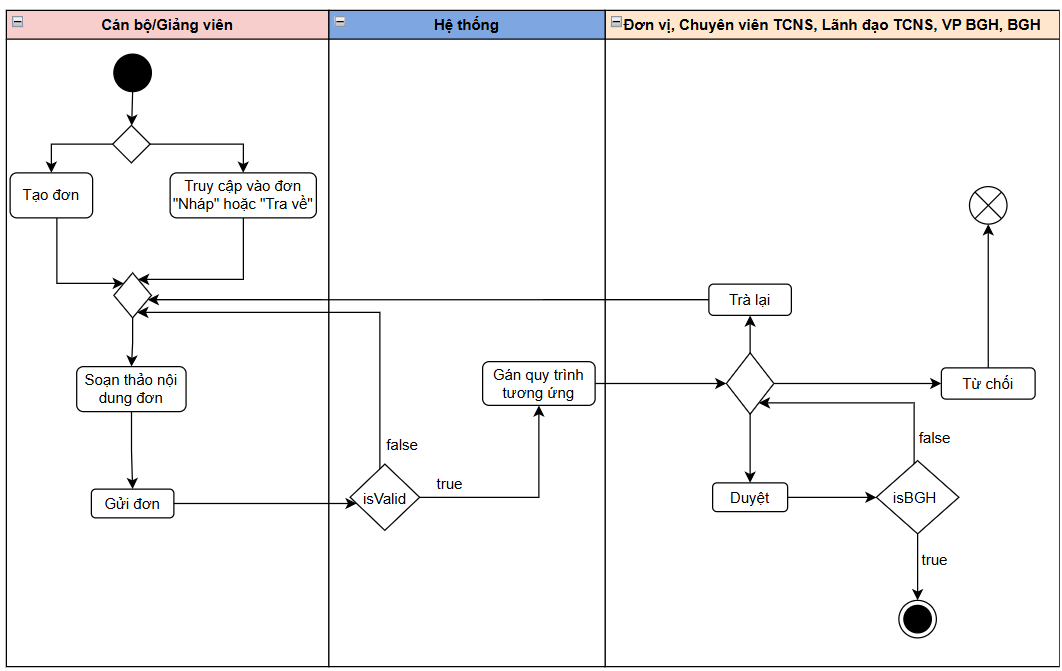
\includegraphics[width=\linewidth]{image/uml/bt_activity.png}
    \caption{\textit{Sơ đồ hoạt động quản lý công tác}}
    \label{fig:BT_AC}
\end{figure}

\subsubsection{Biểu đồ tuần tự}
\begin{figure}[H]
    \centering
    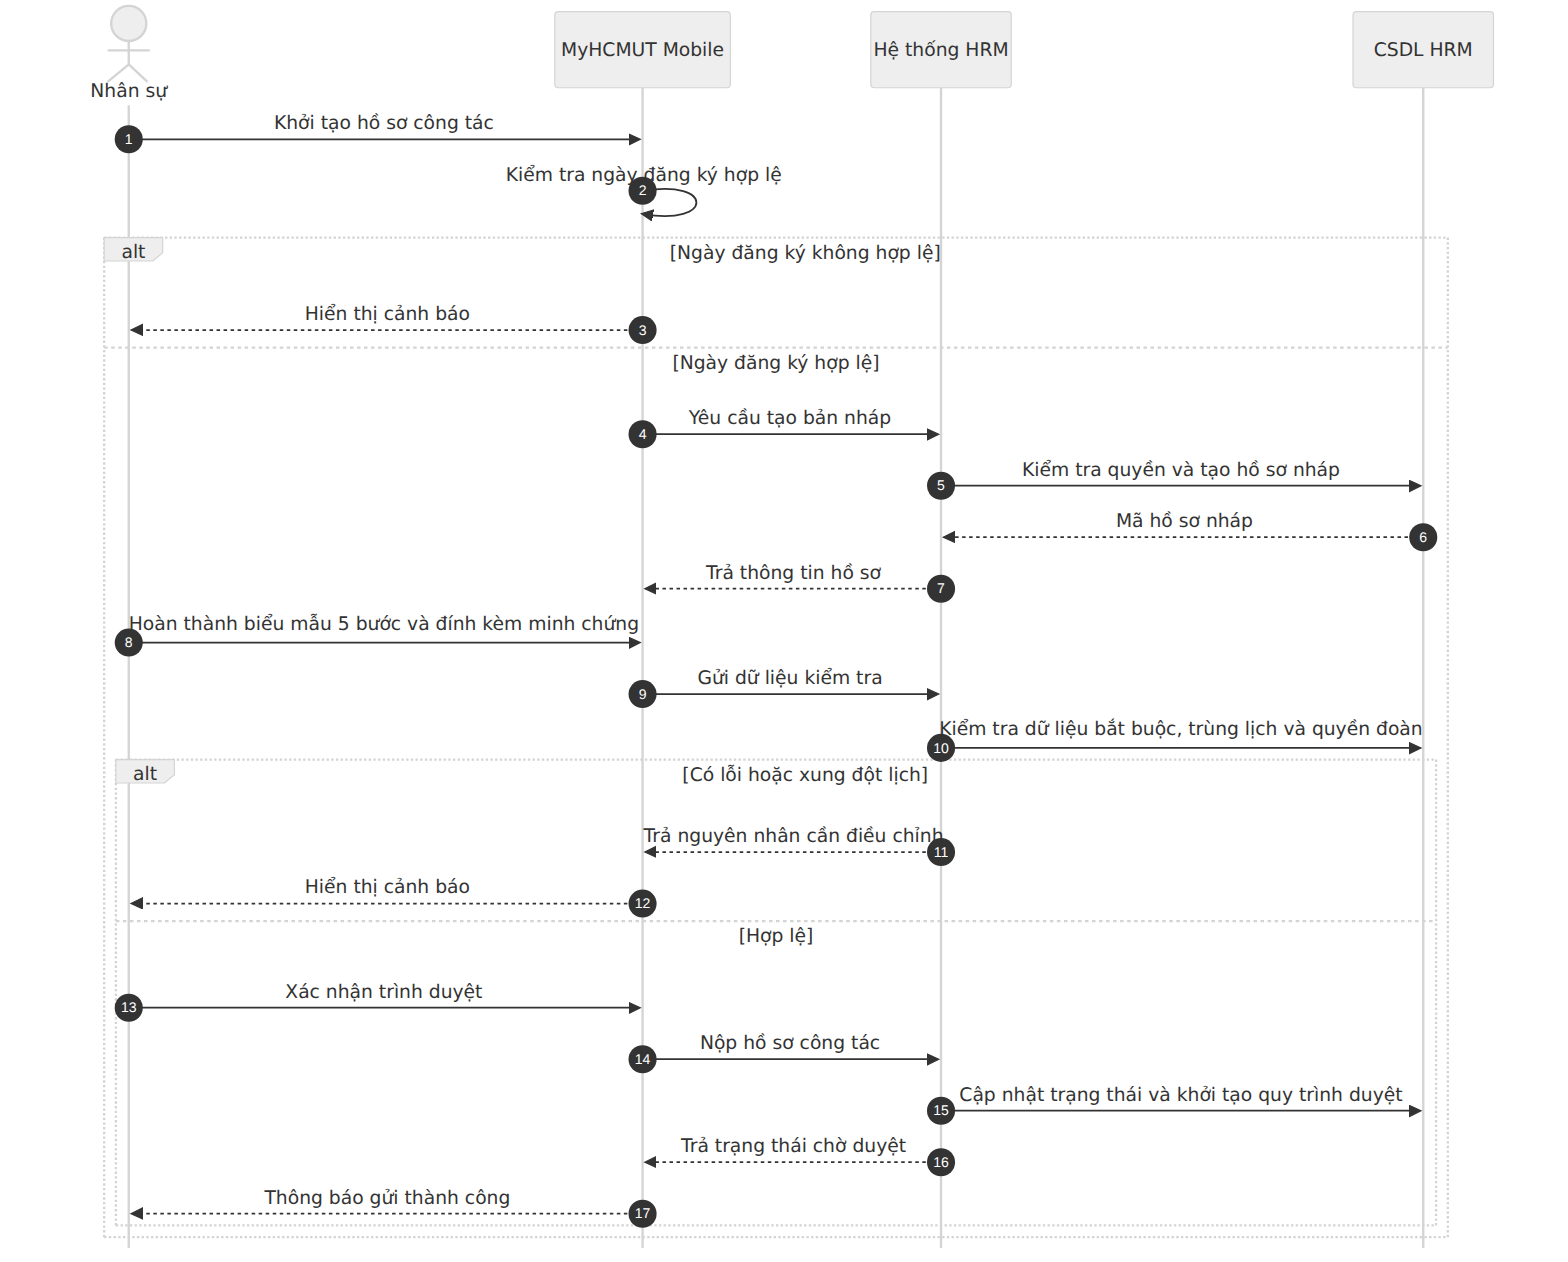
\includegraphics[width=\linewidth]{image/uml/seq_trip_submit.png}
    \caption{\textit{Sơ đồ tuần tự quản lý công tác}}
    \label{fig:BT_SEQ}
\end{figure}
